% 2nd-iso-wiki.tex
% ref: https://tex.stackexchange.com/a/482372/23098

\documentclass[tikz]{standalone}
\usetikzlibrary{shapes,fit}

\begin{document}
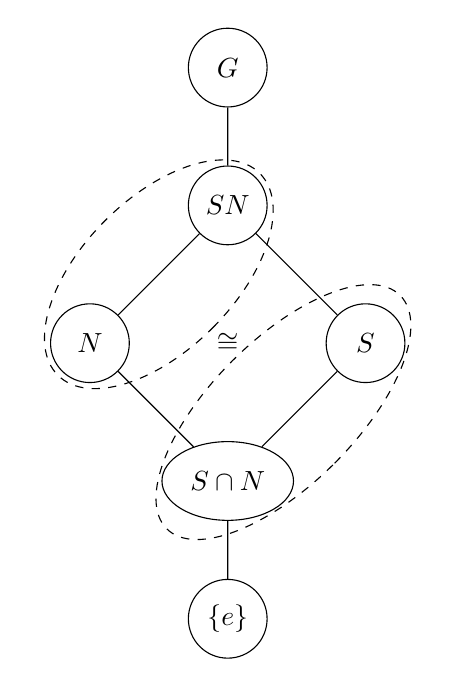
\begin{tikzpicture}[x=1.75cm,y=1.75cm]
  \begin{scope}[every node/.style={draw,circle,minimum size=1cm}]
	\node (g) at (0,2) {$G$};

	\node (sn) at (0,1) {$SN$};

	\node (n) at (-1,0) {$N$};
	\node (s) at (1,0) {$S$};

	\node[ellipse,draw,minimum height=1cm] (scn) at (0,-1) {$S \cap N$};

	\node (e) at (0,-2) {$\{e\}$};
  \end{scope}

  \draw (g)--(sn)--(n)--(scn)--(e) (scn)--(s)--(sn);

  \node[rotate=-45,ellipse,draw,dashed,inner xsep=-7mm,inner ysep=-1mm,fit=(sn)(n)] {};
  \node[rotate=-45,ellipse,draw,dashed,inner xsep=-9mm,inner ysep=1mm,fit=(scn)(s)] {};

  \node {$\cong$};
\end{tikzpicture}
\end{document}
